%% This is an article based on superfri.cls class file of
%% ``Supercomputing Frontiers and Innovations. An International Journal''
%% http://superfri.org/.

\documentclass{superfri}
\usepackage{graphicx}
\usepackage[hidelinks]{hyperref}

\usepackage{todonotes}
\usepackage{cleveref}
\usepackage{subcaption}
\usepackage{comment}
\usepackage{float}

\newcommand{\jk}[1]{\todo[inline]{JK: #1}}
\newcommand{\lr}[1]{\textcolor{blue}{LR: #1}}
\pagestyle{plain}

% ------------
\bibliographystyle{superfri}

\begin{document}

\author{}
%\author{Julian M. Kunkel\footnote{\label{uread}University of Reading, Reading, United Kingdom}\orcidID{0000-0002-6915-1179} \and Luciana R. Pedro\footnoteref{uread}\orcidID{0000-0001-8365-6264}
%}

\title{Potential of I/O-Aware Workflows in Climate and Weather}

\maketitle{}

\begin{abstract}%
The efficient, convenient, and robust execution of data-driven workflows and enhanced data management are key for productivity in scientific computing.
Traditionally, in HPC, the concerns of storage and computing are separated and optimised independently from each other and the needs of the end-to-end user.
As climate and weather workflows become increasingly complex and blend beyond data centres while, at the same time, storage hierarchies become deeper, the community investigates means to re-organise storage access to utilise such environments fully.

The key contributions of this paper are:
1) we sketch the visions of an integrated data-driven approach and discuss the challenges and implications of this strategy, and 2) we illustrate architecture and roadmap that allows the seamless integration into current climate and weather workflows.
The tools employed here to achieve this extended workflow are Cylc, XIOS, DDN IME, and ESDM.

We believe workflows composed of data, computing, and communication-intensive tasks should drive the interfaces and hardware configurations to best support the programming models.
The changes proposed here increase the opportunity of implementations for smarter scheduling of computing and storage in heterogeneous storage environments.

\keywords{workflow, climate, weather, heterogeneous storage, data-driven}
\end{abstract}

% -----------------------------------------------------------------------
\section{Introduction}  // superfri template requires section*
\label{sec:intro}

High-Performance Computing (HPC) harnesses the fastest hardware components to enable the execution of tightly coupled applications from science and industry.
Typical use-cases cover the numerical simulation of physical systems and the analysis of large-scale observational data.
In the domain of climate and weather, there is a considerable demand for the orchestration of ensembles of simulation models and the generation of data products.
A weather forecast service such as ECMWF generates .... \jk{Cylc team, please provide some facts}
Likewise, ensembles in climate can ...

Based on their needs, the climate and weather community has developed a software ecosystem that supports them to execute their large-scale workflows.
While the current advances correspond to a big leap forward, many processes still require experts.
For example, porting a workflow from one system to another still requires adjusting runtime parameters of applications and deciding on how data is managed.
Since performance is of crucial importance to large-scale workflows, careful attention must be paid to exploit the system characteristics of the target supercomputer.
For instance, a data-driven workflow may benefit from using a heterogeneous set of computing and storage technology at the same time.
To obtain the best performance, a specific supercomputer typically requires substantial changes to the workflow to tailor it to the particular machine.

Knowing the capabilities, interfaces, and performance characteristics of individual components are mandatory to make the best use of them.
As the complexity of systems increases and alternative storage and computing technologies provide unique characteristics, it becomes increasingly difficult even for experts to manually optimise resource usage in workflows.
In many cases, modifications are not performed because: 1) They are labour intense: any change to the workflow requires careful validation which may not pay off for small scale runs, and 2) Users are not aware of the potential of the complex system.

In this paper, we illustrate how knowing the Input/Output (I/O) characteristics of workflow tasks and overall experimental design help to optimise the execution of climate and weather workflows. The access of this information may increase the performance, throughput and cost-efficiency of the environments, providing an incentive to users and data-centres that cannot be neglected any longer.
Our approach intends to reduce the burden on researchers and, at the same time, optimise the decisions about jobs running on HPC systems.
Once we have an automated decision about where the job will run and how the storage will be managed, climate and weather scientists can then run their workflows in any machine efficiently without prior knowledge about its architecture.

\section{Workflows in Climate/Weather}
\label{sec:workflows}

In this section, we describe how the environment workflows are executed in a typical software stack.

\subsection{Data Center Infrastructure}

To satisfy the needs for different workflows, data centres are providing a infrastructure consisting of computing and storage devices with different characteristics which makes them more efficient for specific tasks.
Take, for example, the supercomputer Mistral at DKRZ that consists of 3,321 nodes.
It offers two types of compute nodes equipped with different CPUs and a range of GPU nodes.
Each node provides an SSD for local storage, and DKRZ has additionally two shared Lustre file systems with different performance characteristics.
Individual users and projects are mapped to one file system explicitly, and users can access it as work or scratch file system. While data is kept on the work file system indefinitely, its available space is limited by a quota.
The scratch file system allows storing more data, but data is automatically deleted after some time.

Future centres are expected to have even more heterogeneity. A variety of accelerators (GPU, TPU, FPGAs), active storage, in-memory, and in-network computing technologies provide storage and processing capabilities.
\figref{pic/system} shows such an environment with a focus on computation and storage.
Some of these technologies might be local to specific compute nodes or globally available.
Depending on the need, the storage characteristics range from predictable low-latency (in-memory storage, NVMe) to online storage (SSD, HDD), and cheap storage for long-term archival (tape).
\jk{Mention BBs, e.g., DDN IME}
Naturally, the variety of tasks executed by a single workflow may benefit from the different storage and computing infrastructure.

\fig{width=0.6\columnwidth}{pic/system}{Example of an heterogeneous HPC landscape}

\subsection{I/O Stack of a Parallel Application}

\fig{width=0.2\textwidth}{pic/layers-xios}{I/O path for an MPI-parallel application}

A typical I/O stack for a single parallel application like a climate model is shown in \figref{pic/layers-xios}.
In our example, we assume the application is parallelised for performance reasons using MPI.
It may use XIOS to gather data from individual fields which then uses NetCDF4 to store the data as a file.
XIOS provides a domain-level semantics and ...\jk{TODO}

Under the hood, NetCDF4 uses the HDF5 API and file format.
Internally, HDF5 uses MPI again and its data types to specify the nature of the data stored.
Finally, data is stored on a parallel file system like Lustre which, on the server-side, stores data in the local file system as block devices on storage media such as SSDs and HDDs.

Different applications involved in a workflow may use a different I/O stack to store their outputs.
Naturally, the application that inputs previously generated data must use a compatible API to be able to read the specific data format.
In this figure, for example, XIOS is beneficial\lr{beneficial?} for parallel I/O and a process might directly rely on the NetCDF API to read previous data.

Within ESiWACE, we are developing ESDM, ... \jk{TODO}

\subsection{Software Stack}

The appropriate software stack involved in executing a general workflow is depicted in \figref{pic/stages}.
As a preliminary, the user has to specify a configuration representing the workflow and provide scripts for the individual tasks to be executed. After that, the user enacts a workflow engine to start the workflow.
In the following, each stage of the execution is further described.

\fig{width=0.8\textwidth}{pic/stages}{Software stack and stages of execution}

\begin{enumerate}

  \item \textbf{Scientist} specifies a configuration representing the workflow and provides scripts for each task.

  \item \textbf{Workflow Engine} parses the workflow configuration file, generate tasks dependencies, defines a schedule for the execution, and monitors the progress of the workflow.
  Once a task can be executed (dependencies are fulfilled), the workflow engine generates a Slurm script on the fly with the required metadata that will load the user-defined script for each task. Then, Slurm queues the job.

  \item \textbf{Slurm} plans the execution of the job, considering the scheduling policy of the data centre.
  Once the job is ready to be dispatched, i.e., resources are available, and the job priority is the highest, it is started on the supercomputer.

  \item \textbf{Job} runs the user-provided script on one single node assigned by Slurm.
  The script set environment variables containing information about the execution (e.g., a task in the workflow) and the Slurm job (e.g., number of nodes).

  \item \textbf{Script} typically consists of multiple fine-grained commands to create a filename with a template provided by the user. The information is fed into the application which, ultimately, defines the storage location.
%  and may even call multiple parallel applications.

  \item \textbf{Application} runs taking the generated filenames that the script has set.
  The user-specified parallel application may use XIOS or NetCDF to perform the I/O.

\end{enumerate}

\subsection{Cylc}

\lr{Intro}

Cylc is in charge to execute and monitor workflows in which each step is submitted to the batch scheduler of a data centre.
 %, and the relevance of heterogeneous infrastructure to run workflows.
%We focus on high-level considerations to illustrate mandatory concepts.

Consider the Cylc workflow for a toy monthly cycling workflow in \figref{pic/cylc1} \cite{8675433}.
In this workflow, a warm-cycled atmospheric model (\textbf{model}) simulates the physics from a current state to predict the future after a timestep, for example, six hours.
This process is repeated in the model to simulate month and years into the future.
Once the simulation of any month is computed, the data for this month becomes available and can be analysed.
A user has specified the detailed workflow in a Cylc configuration file (\texttt{conf.rc}).
In this workflow, the \textbf{model} is followed by postprocessing (\textbf{post}), forecast verification (\textbf{ver}), and product generation (\textbf{prod}) tasks.
Also, consider, in addition, a task \textbf{check} that compares some verification metric against products from two cycles earlier.\lr{Needed?}

\fig{width=0.9\columnwidth}{pic/cylc1}{Example workflow}

\figref{pic/cylc1} presents the workflow and the dependencies among the tasks, but it is missing the information about I/O and storage.
Decisions about storage must take into consideration the architecture in which the workflow will run.
The developers make the configuration about parallelism and where the data is stored in a script file that is executed for each specific task.

\subsection{Data Management}
\label{sec:datamanagement}

Usually, the scripts for tasks in climate and weather workflows define how the data is stored on the available system.
What happens in many current workflows is that they ignore the benefits of using multiple file systems concurrently and exploiting the data locality between tasks to co-locating them.
On top of that, in the current state-of-the-art, scientists have to optimise the available storage resources intuitively and insert the information about this decision-making process manually.
Once we have the complete knowledge about how the workflow is expected to run, we can optimise steps that were before predefined by the user, usually considering only options for feasibility.

Consider, for instance, one machine with three file systems: a fast \textbf{scratch} file system on which data may reside only for a week, a slower \textbf{work} file system, and each node has a \textbf{local} file system.
What happens in many current workflows is that they only use \textbf{work} and \textbf{scratch}.
When a task is set to computing, the corresponding dataset is moved to \textbf{scratch}, processed, and the resulting datasets are transferred back to \textbf{work}.
If the \textbf{scratch} filesystem achieves its capacity, the datasets move back to \textbf{work} and keep running the task until it is finished which might be inefficient.
If the I/O planning is made a priori, this situation can be avoided.
In addition to the file systems described, many supercomputers also have available for the user \textbf{scratch2} file systems (sometimes local and global).
Therefore, in a real scenario, if the architecture of the machine is known, we can better utilise its resources.

\figref{fig:lifecycle} shows three possible life cycles and the access pattern for a specific dataset.
As shown in \figref{fig:lifecycle1}, the dataset could be stored on the \textbf{local} storage first to avoid congestion on the \textbf{work} file system, then be migrated to \textbf{work} file system where subsequent tasks of the workflow may read it multiple times.
In the end, this dataset might be an intermediate product that can then be deleted.
Alternatively (\figref{fig:lifecycle2}), the dataset could be stored on the \textbf{scratch} file system immediately and accessed there.
However, that would require that the last read access happens before files on \textbf{scratch} are automatically removed.
The last scenario (\figref{fig:lifecycle3}) presents the case where the dataset is created on \textbf{work} by a task and it is copied to a \textbf{local} node. This local node allows read accesses of subsequent tasks which might be beneficial for small random accesses.
However, it would require that the subsequent tasks are placed on the same machine where data is now stored.
The scientist responsible for the workflow must optimise the available resources intuitively.
These are just examples, and currently, the scientists perform such kind of optimisations manually.

\begin{figure}[b]
    \begin{minipage}{.33\linewidth}
        \centering
        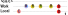
\includegraphics[width=0.9\columnwidth]{pic/lifecycle-1}
        \subcaption{Local and work file systems}\label{fig:lifecycle1}
    \end{minipage}
    \begin{minipage}{.33\linewidth}
        \centering
        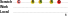
\includegraphics[width=0.9\columnwidth]{pic/lifecycle-2}
        \subcaption{Scratch file system only}\label{fig:lifecycle2}
    \end{minipage}
    \begin{minipage}{.33\linewidth}
        \centering
        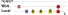
\includegraphics[width=0.9\columnwidth]{pic/lifecycle-3}
        \subcaption{Local and work file systems}\label{fig:lifecycle3}
    \end{minipage}
    \vspace{5pt}
    \caption{Alternative life cycles for mapping a dataset to storage and the operations: \textbf{C}reate, \textbf{M}igrate, \textbf{R}ead, and \textbf{D}elete}
    \label{fig:lifecycle}
\end{figure}

\section{State of the Art}

Manual tiering requires the user or application to control the data placement, i.e., storing data (typically in the form of files on a particular storage system) and, usually, moving data between storage by using scripts.
One limitation here is that decisions about how data structures are mapped and packaged into files are made once by the producing application, and cannot be changed without manual intervention by a downstream application.

A policy system (e.g., deployed on a burst buffer) aims to simplify the data movement for the user, but typically migrates objects in the coarse granularity of files.
However, the semantical information that can be used by this type of system to make decisions is limited, e.g., data location, file extension, age of the file, etc.

Other tools for workflow handling, how is this information transported?

dataspaces + ADIOS + in-situ

\jk{TODO}

\cite{Vladimirov2014FileIO}

Slurm \cite{Jette02slurm:simple}

ESDM \cite{esdm}

Cylc \cite{8675433}

XIOS \cite{xios}

NetCDF \cite{Jenter92netcdf:a}

Compression \cite{TDTSOCAFQC17}

\section{Vision for I/O-Aware Workflows}
\label{sec:vision}

Data system do not respect the importance of data depends at all. Aspects like costs to reproduce the data (can it be reproduced easily), the type of the experiment (test run, production run) and runtime constraints for the overall and potential crucial workflow are not considered.
Value and priority should influence fault-tolerance strategies and imply the quality of service for performance and availability.\lr{kind of lost here too}

There are several approaches to implement the technology for the vision proposed in this work, and changes need to be made to software components to realise it.
In the next sections, we will discuss a specific design for our transitional roadmap considering climate and weather workflows and tools scientists from this field already use in their routine research.
Applied scientists should not spend time understanding hardware characteristics, but using their time to develop their work, let the computer do the job as most straightforward as possible, and just collect and analyse the results.
However, nowadays, to be able to run a job in a HPC environment efficiently, researchers have to develop profound knowledge about their workflow, which is expected, but also about decisions regarding storage, communication, and computing.

We propose an approach to reduce the burden on researchers and, at the same time, optimise the decisions about jobs running in HPC systems.
Once we have an automated decision about where the job will run and how the storage will be managed, scientists can then run their workflows in any machine without further interactions and even without previous knowledge about the machine architecture.
Our vision for I/O-aware workflows requires two additional information. Firstly, the user must augment the workflow description with information about I/O requirements and explicitly annotate dependencies to data sets. Secondly, the data centre (or expert user) must provide details about the storage architecture.

\subsection{Extended Workflow Description}

In general, climate and weather workflows allow specifying tasks and the dependencies among them.
We aim to enable enhancing the current information with characteristics for input, and output, i.e., the datasets.
An example workflow containing input datasets and (intermediate) products is illustrated in \figref{pic/workflow}.
Nodes represent tasks or data, and arrows indicate the dependencies.
In the example, Task\,1 needs two datasets to perform its work, it directly communicates with Task\,2 and produces Product\,1.
Most of the workflow can run automatically, except for the manual quality control of the products and the final data usage of Product\,3.
This last step represents the typical uncertainty of data reuse, i.e., it is unclear how Product\,3 will be used further.
In the approach proposed in this work, each task is annotated with the required input datasets and the generated products must include metadata such as data life cycle information, the value of data, and how long should it be kept.

\fig{width=0.4\columnwidth}{pic/workflow}{Example of a high-level workflow with tasks and data dependencies}

\lr{Replicate this figure and explain the idea of recomputing of data.}

D1 D2 P1 P2 P3 + arrows

D1 + D2 (small) + P1 + P2 (short) + P3 (huge) => P3 might be recomputed

\subsection{System Information}

% Here we focus on utilising a heterogeneous storage environment.
While many optimisations are possible once an abstraction is in place, the optimisations we discuss here are related to the life cycle of datasets and the placement of such datasets into specific storage according to system performance characteristics and the workflow specification.
For achieving that, the system information shall comprise of all available storage systems, the system topology, and details of each of the required components.
Simplified and complex models of the components can be included to approximate performance for specific I/O patterns allowing to predict performance behaviour.
It is expected that the data centre (or expert users) can create such a configuration file, e.g., by using vendor-provided information or by executing benchmarks.
With this information, the I/O scheduler can make the placement and migration decisions for individual datasets and manage their relocation during their life cycle, as discussed in \Cref{sec:datamanagement}.
This separation of concerns allows us to abstract from the workflow what is essential and what a machine should optimise to ensure that the resources available are being used smartly. \lr{Check abstract!}

\subsection{Data Movement}

\subsection{Smarter I/O Scheduling}

In this paper, we focus on utilising a heterogeneous storage environment instead of exhaustively discussing the potential that is unleashed with the right level of abstraction in place. Researchers are welcome to exploit the available opportunities.\lr{Lost.}

\lr{Combine next two paragraphs}

Consider the hypothetical case of having just two tasks A and B that need to be repeated many times.
Datasets generated by Task\,\textbf{A} are used by Task\,\textbf{B} and hence both tasks must have access to the same data in the system.
Because there is one script responsible for setting the configuration, the decision in which directory to store data is somewhat fixed.
Such configuration was done manually and with restricted information about the storage and system architecture.
It would be interesting to explore storage options for the datasets and, e.g., have different cycles placed in different storage systems.
If the lifetime of such dataset is, for instance, two cycles, alternate the datasets into two scratch file systems is something that would be a simple job for an I/O-aware scheduler.
However, currently, that implies in having at least two scripts\footnote{Complicated scripts would have allowed changing the storage type depending on the cycle. Still, it is a significant burden to the user.} for each task with information about the different storage placement.

\figref{pic/cycle4} exemplifies a restriction of our example climate/weather workflow the way it was being generated.
Assume you have, for instance, five cycles of the model running with all the necessary post-processing steps.
Typically, the user has written the scripts for each task by defining a filename using the same prefix that places the dataset at the same storage type every time.
That happens because all datasets generated by Task \textbf{model} will be used by Task \textbf{post\,prod}, so they should stay on the same node.
The user-specific storage locations are a viable option to run a workflow.
The user might even have analysed various scenarios such as depicted in
Section \ref{sec:datamanagement}.

Additionally, by knowing how to rerun the workflow behind the data creation, a smarter storage system could trade data security with potential recomputation opportunities to optimise the cost-efficiency of the system.
Intermediate states could be rerun by utilising virtualisation and container technologies.
Similarly, the scheduler may decide to couple subsequent steps of a workflow directly without storing intermediate data products on persistent storage.
Finally, data might be replicated by enabling the system to rerun parts of the workflow in case of a data loss.

Ultimately, by abstracting and automatising the workflow, we provide a smarter route taking into consideration the architecture available and the way the datasets are stored during the intermediate steps of the workflow.

\fig{width=0.8\columnwidth}{pic/cycle4}{Five stages workflow example}

\lr{Color the pic and change the definition of the other pic.}

\subsection{Benefit}

The benefits of the proposed vision are:

\begin{description}

\item[Abstraction] The user does not have to know the architecture that the workflow will run, removing the specialist from the decision-making process.

\item[Optimisation] The workflow will be optimised specifically for the available system infrastructure considering potentially runtime characteristics and storage resilience which will increase performance and system utilisation.
By knowing the workflow behind the data creation, the system could even trade data security with potential recomputing opportunities to optimise the cost-efficiency.

\lr{Introduce the picture as an example?}

\item[Performance-portability] The user has to specify the I/O requirements only once for the tasks of a specific workflow, and the workflow can now run on any system without user intervention.
Even more, if the system characteristics change, e.g., it gets upgraded, an additional storage tier becomes available, or if storage degrades, the I/O-aware workflow could automatically adapt and make use of this new environment.

\end{description}

\section{Design}

This section describes our first approach to incrementally extend the current software stack for climate and weather workflows which realises parts of our vision.
To automatically make scheduling decisions, the software stack needs to:

\begin{enumerate}

\item Delivers information about storage life cycle together with the workflow, and

\item Adapts the resulting workflow, individual scripts and application executions to consider the adaptative I/O scheduler.

\end{enumerate}

\lr{What comes next...}

\subsection{Agregatting Data Dependencies}

\figref{fig:cycle1} introduces one cycle of the workflow in \figref{pic/cylc1} with a simplified notation. The arrows represent the tasks dependencies, but there is no information about data that are generated. Tasks \textbf{verification} and \textbf{post\,proc} depend on Task \textbf{model}, but does Task \textbf{model} needs to be fully completed to satisfy the dependencies?
Of course, once Task \textbf{model} is completed, the dependent tasks can be executed, and that is the type of information Cylc has to create to reproduce the workflow.

\begin{figure}[b]
    \begin{minipage}{.45\linewidth}
        \centering
        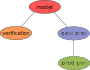
\includegraphics[width=0.9\linewidth]{pic/cycle1}
        \subcaption{Including tasks and dependencies}\label{fig:cycle1}
    \end{minipage}
    \begin{minipage}{.45\linewidth}
        \centering
        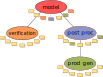
\includegraphics[width=0.9\linewidth]{pic/cycle-io-dep}
        \subcaption{Including tasks, datasets and dependencies}\label{fig:cycle-io-dep}
    \end{minipage}
    \vspace{5pt}
    \caption{Example of a high-level workflow}
    \label{fig:cycle}
\end{figure}

\lr{Think about split the colours.  }

The scenario presented in \figref{fig:cycle-io-dep} shows the same cycle of \figref{fig:cycle1}, but extended information about datasets is added.
In this picture, we have the tasks dependencies, and we explicitly list the datasets dependencies regarding the tasks that generated them.
The way data moves through tasks is by creating datasets to pass on the information, including filename and storage destination.
The datasets produced by every task are coded in the workflow scripts before Cylc evaluation, and it is just replicated by this tool. The tasks can create a different number of datasets, and these datasets may be necessary for the immediate next task in the current cycle, or tasks in different cycles.

Datasets colours indicate which task will use their information and datasets in yellow represent information that will be used in a different cycle. From the diagram we can also notice that Task \textbf{model} will generate one dataset for Task \textbf{post\,proc}, one dataset for Task \textbf{prod\,gen}, two datasets for Task \textbf{verification}, and three datasets for later cycles. The tricky part when we consider only tasks and not the datasets in the workflow is that it may lead to the false impression that one task depends only on the immediately previous one. Note, for instance, that one dataset produced by Task \textbf{model} is later used in Task \textbf{prod\,gen}. That is not an immediate conclusion when we analyse just the arrows for the dependencies among tasks. It is clear that Task \textbf{model} is a dependency for Task \textbf{post\,prod}, which is then a dependency for Task \textbf{prod\,gen}. Still, the crucial information here is that any dataset being used in the current cycle can also be used later.

The access to this information before the process starts can be used to optimise where compute jobs will be executed and how these datasets will be stored during the workflow.
This information today is static and manual, leaving open opportunities for automatisation and optimisations.
The idea here is to embrace the concept that tasks dependencies are really imposed by datasets dependencies.
Once we insert the datasets explicitly in the workflow, it is easier to see that many optimisations regarding storage can be made.

\subsection{Extended Workflow Description}

The user now has to provide information about datasets required for input and the generated output for each Cylc task in a separate file similarly to Cylc's workflow configuration file.

\begin{description}

  \item[Name] The name of the field generated/required, which may include a pattern such as supported by Cylc.

  \item[Size] An estimate of the file size.

  \item[Lifetime] How long the data must be retained on storage (if at all).

  \item[Type] It may specify the type of data, i.e., checkpoint, diagnostics, temporary.

\lr{Sketch a config file based on Cylc}

\end{description}

\subsection{System Information}

The information about the system is provided using a configuration file for ESDM.

\lr{Insert esdm.conf and explain.}

\subsection{Smarter Scheduling}

ESDM has already an interface with NetCDF. The ESDM Scheduler will make the schedule, and it can be used in different steps of the process. Assuming the user can provide extra information in advance, ESDM can interact in the process before the user gives the data to the Cylc tool, using the gathered information to construct a temptive optimised workflow. Once Cylc builds the workflow, ESDM can interact again after the configuration of the scripts for both effective and efficient run of the parallel applications regarding the available storage and architecture.

\lr{Explore potential for migration using IME.}

\subsection{Modified Software Stack}

The proposed I/O-aware scheduler, called here EIOS (ESDM I/O Scheduler), is now introduced.
The appropriate software stack involved in executing a workflow with EIOS is depicted in \figref{pic/stages-io}.
The suggested alterations can be seen in boxes pointed by red arrows, and the remaining components are the current state-of-the-art for general workflows (\figref{pic/stages}).

The end-user has now to provide an additional file that covers the I/O information for each task, and slightly changes (discussed below) have to be made to the current scripts``.
Here, we use ESDM as the middleware that aims to exploit heterogeneous system environments and Cylc as the workflow engine.
In the following, we describe the modifications we propose in this vision paper for each stage of the software stack.

\fig{scale=1.4}{pic/stages-io}{Software stack and stages of execution with our I/O-aware scheduler -- EIOS}

\begin{enumerate}

  \item \textbf{Scientist} In addition, now the user also has to provide data dependencies and characteristics of the datasets and products generated.

  \item \textbf{Cylc} EIOS is invoked by Cylc to identify potential optimisations in the schedule before generating the Slurm script.
  EIOS may decide that subsequent jobs shall be placed on the same node, reorder the execution of some jobs, and provide information for conducting data migration.

  \item \textbf{\color{red}{EIOS}} The ESDM I/O Scheduler reads the information about the workflow (original and I/O workflow configuration files) and acts depending on the stage of the execution.
  EIOS consists of several subcomponents:
    \begin{itemize}

      \item The high-level scheduler that interfaces with Cylc.\\

      \item A tool based on Cylc to generate pseudo-file names used by applications with ESDM support.\\

      \item A data management service (not shown on the figure) that migrate and purge data according to information from EIOS, e.g., the user life cycle specification.\\

    \end{itemize}
  EIOS components use ESDM through the \texttt{esdm.conf} file \ref{aa}. This file contains information about the available technology in the data centre and its I/O characteristics to make decisions about `how to prioritise I/O targets.

  \item \textbf{Slurm}
  Cylc may now have added an optimisation identified by EIOS and that is now handled by a modified Slurm.
  Also, if migrations have to be performed, Slurm will administer them according to the specification in the job script.

  \item \textbf{Job}
  A job might run on the same node than a previous job to utilise local storage. \lr{+migration}

  \item \textbf{Script}
  Filenames are now generated by a replacement command that calls EIOS to create a pseudo filename.
  This filename will encode additional information for ESDM about how to prioritise data placement according to data access.

  \item \textbf{Application}
  The application may either use XIOS, NetCDF with ESDM support or ESDM directly to access datasets.
  Hence, in \figref{pic/layers-xios}, the HDF5 layer is replaced with ESDM.
  ESDM loads the \texttt{esdm.conf} file that contains the information about the available storage backends and their configuration.
  ESDM extracts the long-term schedule information from the generated pseudo filenames and employs it during the I/O scheduling to optimise the storage considering data locality between tasks.

\end{enumerate}

\section{Conclusions}
\label{sec:conclusions}

The changes proposed in this work increase the opportunity for smarter scheduling of computing and storage in heterogeneous storage environments considering characteristics of workflows and data.

Organising the data placement on storage tiers is typically performed manually by the developer/user or via policies, leading to suboptimal optimisations.

Manual and hard-coded workflows cannot handle changes in the environment. On top of that, it is a tedious, non-portable, and error-prone task.
Any hard-coded decision has significant implications for the performance of both applications and systems because the optimal choices about file size and content may be very different for data production and any subsequent data analysis phase.
By increasing the abstraction level for scientists, not only tedious manual optimisation could be automatised, but also novel strategies for further optimisations can be harnessed.
Therefore, users must be able to express their workflows in an abstract fashion that allows the system to generate (near-)optimal execution plans and monitor their execution.

\section*{Acknowledgements}

\small
This project is funded by the European Union's Horizon 2020 research and innovation programme under grant agreement No. 823988.

\openaccess

\bibliography{paper}
\end{document}

Machine Learning has been proven effective in replacing human-beings, and it may also adapt the workflow dynamically in case of unexpected situations (the system is down, nodes are unresponsive, etc.).

(3.3)

By monitoring I/O accesses, we can automatically draft such I/O descriptions on behalf of the user to simplify the specification.
All we need is to run one cycle of the specific workflow, considering that a workflow cycle is executed many times in climate and weather; this is a cheap approach.
From the recorded I/O accesses, we analyse the I/O patterns and dependencies associated with it to generate the configuration file.

\cite{TUIBIHWLSC19}

3.2 end

- Collect all ideas and enumerate them.

- Decide on what we can actually will do.

Potentially, EIOS may generate an \texttt{esdm.conf} file for the specific application to adjust the mapping of data to available storage targets.
